\subsection{Show the user that you are trustworthy}

Trust between your site and your users is essential.
Therefore you have to guarantee the protection of user privacy and promise that user data will be used only for specific purposes that the user clearly agrees to.
We must minimize the risk of disclosing user data, and maintain user safety, confidentiality and integrity of information.
For this we must follow both the legal norms and an ethics of good practices.
Do not require user identification merely to show general information.
Always ask for permission to capture data and make clear what it will be used for.

\subsubsection*{Suggested strategies} 

\begin{itemize}
    \item Use secure platforms, such as SSL if you develop a web application.
    \item If you use third-party APIs, make sure to check the level of security they offer.
    \item Implement a system that does not allow linking the data with a user.
    \item Tell the user why you need their data, and how you will use it.
    \item Give the user the possibility to delete their data if they wish.
\end{itemize}

\subsubsection*{In the context of Aire Guru \ldots} 

In our case, security is high, since for our main purpose, personal history
of exposure to contamination, it is not essential to collect the user's details.
SSL has been used to achieve a level of competent security, which guarantees the encryption of
the information sent through the network.\\

For the identification of the user we use Firebase, which is a commonly used, secure, and proven API.
This API provides us with an identifier, which may be encrypted.
When the data reaches our database, we verify the user identity and then re-encrypt the user with our own salt to
ensure that it is not possible to correlate the Firebase identification with our database. \\

We never store the users exact location, only a containing polygon derived from the sensor coverage.
We have also implemented a time limit, which allows us to have the necessary precision to show exposure to pollutants, but doesn't allow user tracking.\\

We never collect the user's position without their permission.
To get this permission, we require an explicit action - the user has to select "Mi ubicacion" (My location) and accept that we may determine their position.
Of course the user can always revoke this permission and delete their data at any time. \\

During the post-launch survey, some users indicated that they would prefer to create an account with a username and password rather than use their email accounts, for fear of "information theft".
We have not yet done this. \\

\begin{figure}[ht]
    \centering
    \subfigure[Location Access]
        {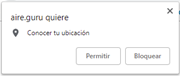
\includegraphics[width=5.5cm]{Figure_6_3_1_a_locationAccess}}
    \hfill
    \subfigure [Settings]
        {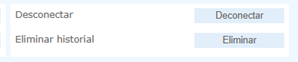
\includegraphics[width=5.5cm]{Figure_6_3_1_b_settings}}
    \caption{Filters}
\end{figure}

\begin{center}
    \bf{ (a)Location Access (b)Settings\\

    Figure 6.3.1. Filters}
  \end{center} 

% The collection of locational data is not exhaustive, but guarantees accuracy. \\

As we want a transparent website, we explain to the user that we need their data before
they are identified, and of course, the identification is optional. \\

\begin{figure}[ht]
    \centering
    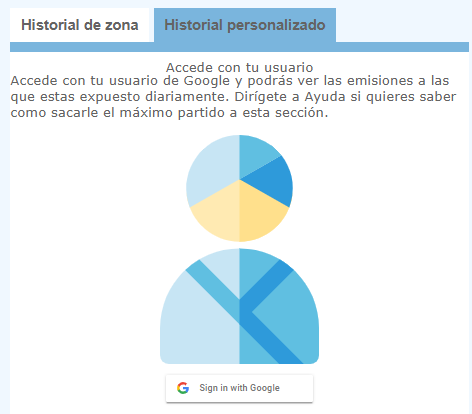
\includegraphics[width=8cm]{Figure_6_3_2_loginInfo}
    \caption{Info before login}
\end{figure}
\begin{center}
    \bf{ 
    Figure 6.3.2. Info before login}
  \end{center} 